
\chapter{Introduzione}


La crittografia è un metodo per un utente di condividere in maniera sicura i propri dati su un mezzo di comunicazione o un sito insicuri.\\
Prima della crittografia a chiave pubblica, un metodo ampiamente utilizzato tra due utenti per comunicare informazioni confidenziali era quello di stabilire a priori un segreto comune e ben protetto che permettesse di decodificare le informazioni.\\
Nonostante questo metodo sia accettabile per piccoli gruppi diventa obsoleto ed inutilizzabile in un'infrastuttura molto grande come quella di Internet che conta miliardi di utenti.\\

Quasi 40 anni fa, Diffie ed Hellman pubblicarono una rivoluzionaria idea racchiusa nel concetto di \textbf{crittografia a chiave pubblica}:\\
{ \itshape ``due persone possono comunicare in maniera sicura \emph{senza} dover accordarsi su un segreto comune.''}\\
\begin{center}
\begin{tikzcd}
\begin{tabular}{@{}c@{}}Alice\\sceglie\end{tabular} \quad a \arrow{r} & \begin{tabular}{@{}c@{}}Alice\\calcola \end{tabular} \quad A = g^a \arrow{ddr} & \begin{tabular}{@{}c@{}}Alice\\calcola\end{tabular}  B^a = g^{ab} \arrow{dr} & \- \\
\begin{tabular}{@{}c@{}}Gruppo ciclico $G$\\e gen. $g$\end{tabular} \arrow{u}\arrow{d} & \- & \- & \begin{tabular}{@{}c@{}}Segreto\\comune \end{tabular}\quad g^{ab} \\
\begin{tabular}{@{}c@{}}Bob  \\sceglie\end{tabular} \quad b \arrow{r} & \begin{tabular}{@{}c@{}}Bob  \\calcola \end{tabular} \quad B = g^b \arrow{uur} & \begin{tabular}{@{}c@{}}Bob  \\calcola\end{tabular}  A^b = g^{ab} \arrow{ur} & \- 
\end{tikzcd}
\end{center}

Una terza persona che osserva lo scambio di chiavi tra Alice e Bob conosce completamente il sistema ma deve ottenere o $a$ o $b$ per poter ottenere il segreto comune. Per questo motivo dovrà risolvere una delle due equazioni
\[ g^a = A \qquad \text{oppure} \qquad g^b = B \]
Questo calcolo è chiamato \emph{logaritmo discreto} e non esiste alcun algoritmo efficiente per risolverlo.\\
Per questo motivo il metodo è \emph{``pubblico''}:\\
sia Alice che Bob scelgono il proprio segreto che poi comunicano in maniera protetta su un canale completamente pubblico.\\
A questo punto raccogliendo le informazioni condivise sul canale, Alice costruirà il segreto comune \textbf{senza} conoscere quello personale di Bob.
\vspace{0.4cm}

Al giorno d'oggi la crittografia a chiave pubblica è uno strumento fondamentale e il suo utilizzo è centrale per la comunicazione sicura via web, per la cifratura di dispositivi d'archiviazione e per la possibilità di garantire l'autenticità di persone mediante firma digitale.\\[0.2cm]


Vi sono delle particolarità per questa tipologia di crittografia:
\begin{itemize}
	\item Crittare è un metodo per inviare un messaggio ad \textbf{una singola} persona che detiene una chiave segreta
	\item L'accesso ai dati cifrati è totale o nulla: una persona può decifrare e leggere completamente il messaggio \textbf{o} non può nemmeno decifrarlo.
\end{itemize}

\vspace{1cm}
Siamo interessati a risolvere un problema formulabile come:

\begin{center}
{\itshape È possibile costruire un sistema crittografico dove sia possibile 
\begin{enumerate}
	\item crittare \textbf{una} volta sola il messaggio \label{critto1}
	\item distribuire alle persone chiavi private capaci di filtrare il contenuto in base alle loro autorizzazioni \label{critto2}
\end{enumerate}
}
\end{center}
\vspace{0.6cm}

Consideriamo degli esempi concreti:
\begin{itemize}
	\item {\itshape un servizio di memorizzazione su Internet che immagazzina immagini per i diversi utenti registrati.\\
Le forze dell'ordine potrebbero aver bisogno di cercare un immagine contenente un particolare volto.\\
Il gestore del servizio ha bisogno di fornire una chiave segreta alle forze dell'ordne che sia in grado di decifrare le immagini che contengono la faccia cercata ma che \textbf{non} visualizzi il resto delle immagini per non compromettere la privacy degli utenti non indagati.}
	\item {\itshape una società televisiva emette in broadcast tutto il suo palinsesto.\\
	Ogni cliente ha la possibilità di comprare \emph{pacchetti} tematici che più preferisce.\\
	All'acquisto, al cliente viene fornita una smart card da inserire nel decoder contenente una chiave privata fornita dalla società televisiva.\\
	L'utente potrà guardare i programmi da lui comprati ma \textbf{non} gli altri.}
\end{itemize}

\vspace{1cm}

Se dovessimo utilizzare la normale assunzione Diffie-Hellman con chiavi pubbliche, avremo ad esempio un sistema di questo tipo:

\begin{center}
\begin{minipage}[c]{0.9\textwidth}
		\centering
		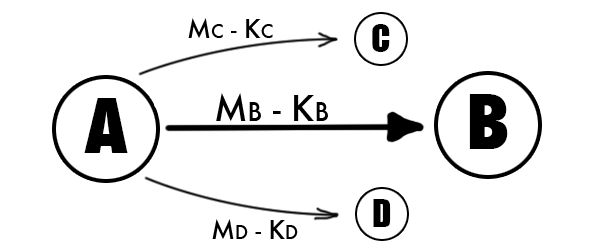
\includegraphics[keepaspectratio,width=\textwidth]{keying.png}\\
		{\small\scshape Un messaggio $M$ deve esser criptato con la chiave $K_I$ per esser mandata all'utente $I$}
\end{minipage}
\end{center}
\vspace{0.4cm}

dove siamo costretti ad avere molte chiavi diverse per permettere la comunicazione verso ogni destinatario. Il messaggio viene crittato tante volte quanti sono i destinatari.\\
Questo metodo non ci permette di risolvere il punto \ref{critto1} del problema.\\[0.3cm]

Per questo motivo, Sahai and Waters \cite{sahai} fanno i primi passi per risolvere il problema intriducendo il concetto di ABE : Attribute Based Encryption.\\
Questo schema prevede la definizione di un insieme di attributi che funzioneranno da \emph{etichettatura} per ogni messaggio crittato.\\
La chiave di decifratura verrà calcolata per ogni utente in base ad una combinazione logica di attributi ben precisa: viene così creata una vera e propria policy d'accesso differenziata per ogni utente che può esser scritta mediante operatori logici AND ed OR.\\[0.4cm]
A questo punto, l'utente è in grado di crittare il messaggio \emph{attaccandogli} gli attributi che preferisce. Questi attributi definiranno quali utenti potranno decifrare il messaggio: le chiavi che rispettano la policy, utilizzando gli attributi del messaggio, hanno diritto e possono decrittarlo.\\[0.2cm]

\begin{center}
\begin{minipage}[c]{0.9\textwidth}
		\centering
		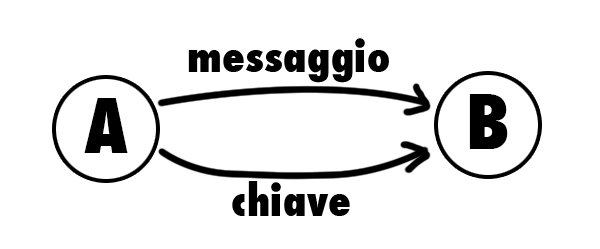
\includegraphics[keepaspectratio,width=\textwidth]{pairing.png}\\
		{\small\scshape Un unico messaggio $M$ etichettato con gli attributi $(1,3)$ viene mandato a tutti gli utenti. Solo gli utenti che detengono una chiave adatta possono leggere il messaggio.}
\end{minipage}
\end{center}

\vspace{0.4cm}

Riprendiamo l'esempio della società televisiva per spiegare il metodo ABE:\\
\begin{itemize}
	\item La società televisiva decide di differenziare il proprio palinsesto utilizzando i nomi dei vari programmi come ad esempio
	\[ \{ \text{ Rugby } , \text{ Film } , \text{ Calcio } , \text{ Mondiali }\} \]
	creando così l'insieme di attributi.
	\item Vengono prese le varie trasmissioni e queste vengono etichettate con gli attributi decisi. Ad esempio un film verrà etichettato con $\{$ Film $\}$ mentre la finale dei mondiali Fifa con $\{$ Calcio, Mondiali $\}$.\\
	Questa fase di etichettatura critta il contenuto.\\
	Il tutto viene diffuso in broadcast.
	\item Il cliente che acquista il pacchetto dei mondiali Fifa, riceverà una chiave privata capace di decifrare le trasmissioni $\{ $ Calcio , Mondiali $ \}$ con una policy \emph{Calcio AND Mondiali}.\\
	\textbf{NON} potrà decifrare le trasmissioni etichettate con $\{$ Film $\}$ o $\{$ Rugby $\}$. \textbf{NON} potrà decifrare quelle unicamente etichettate con $\{$ Calcio $\}$ poiché la sua chiave ha una policy che accetta le trasmissioni con gli attributi Calcio \textbf{AND} Mondiali.
\end{itemize}

\vspace{0.2cm}
Lo schema è quindi capace di risolvere il problema che consideriamo.\\[1cm]

Nello studio di questa tesi, è stato trovato un metodo di crittografia molto simile nella costruzione ma con uno scopo pratico differente:\\[0.3cm]
{\large \textbf{Identity Based Encryption}}\\
\begin{center}
\begin{tikzcd}
\begin{tabular}{@{}c@{}}Alice\\si autentica\end{tabular} \arrow{d} & \begin{tabular}{@{}c@{}}Alice ottiene\\le chiavi\end{tabular} & \begin{tabular}{@{}c@{}}Alice calcola\\la chiave\\pubblica\\di Bob \end{tabular} \arrow{r} & \begin{tabular}{@{}c@{}}Alice comunica\\con Bob\\segretamente \end{tabular} \arrow{dd} \\
\begin{tabular}{@{}c@{}}Ente Garante\\fornisce la\\chiave privata\\dell'utente\end{tabular} \arrow{ur}\arrow{dr} & \begin{tabular}{@{}c@{}}Ente Garante\\fornisce la\\chiave pubblica\\del sistema\end{tabular} \arrow{u}\arrow{d} &  \- & \- \\
\begin{tabular}{@{}c@{}}Bob\\si autentica\end{tabular} \arrow{u} & \begin{tabular}{@{}c@{}}Bob ottiene\\le chiavi\end{tabular} & \begin{tabular}{@{}c@{}}Bob calcola\\la chiave\\pubblica\\di Alice \end{tabular} \arrow{r} & \begin{tabular}{@{}c@{}}Bob comunica\\con Alice\\segretamente \end{tabular} \arrow{uu} 
\end{tikzcd}
\end{center}
 Un garante genera per ogni utente delle chiavi private che vengono concesse unicamente se l'utente viene autenticato.\\
 A questo punto ogni utente autenticato avrà una propria chiave privata e una pubblica del sistema.\\
 Sarà possibile calcolare la chiave pubblica degli altri utenti utilizzando una \emph{frase caratteristica} come il numero di telefono o un indirizzo email. Con queste chiavi è possibile comunicare firmare e crittare i messaggi per poter esser communicati.\\[0.2cm]
 L'identità di una persona definisce la chiave rendendo il modello molto simile alla crittografia a chiave pubblica. È in grado di risolvere il problema principale seppur con qualche problema pratico:\\
quando l'utente ha bisogno di rinnovare la propria coppia di chiavi, quella pubblica non può esser trovata da altre persone utilizzando la frase caratteristica originale poiché essa fornisce la vecchia chiave pubblica.\\[0.2cm]

Questo metodo, ideato temporalmente prima degli altri, risente di difficoltà pratiche che lo rendono inutilizzabile per un applicazione reale.

\vspace{0.2cm}

Altre differenze tra i due schemi si può trovare nella sezione \ref{ibeabe}\\[0.2cm]


Lo strumento principale tra tutte queste costruzioni è un pairing $e$ tra gruppi ciclici. Questo pairing deve avere proprietà particolari (vedi \ref{pairinge}).\\
Esistono pairing complessi \cite{maas} \cite{benoit} tra cui il pairing di Tate e il pairing di Weil.\\[0.2cm]

Lo schema crittografico ABE non è ancora pienamente conosciuto ed è per questo difficile definire e garantire un livello di sicurezza adatto per poter esser utilizzato nella quotidianità, come spiegato nella sezione \ref{secur}.\\[0.2cm]

In questa tesi verrà studiato lo schema ABE descritto nel paper \cite{kpabe} nel seguente modo:
\begin{itemize}
	\item \textbf{Analisi del problema} e definizione astratta degli algoritmi utilizzati e della struttura d'accesso che vogliamo utilizzare.\\
	Definizione dell'algoritmo d'attacco per la definizione dell' assunzione decisionale bilineare di Diffie-Hellman.
	\item \textbf{Costruzione della struttura} d'albero e definizione analitica dei vari algoritmi. Effettiva costruzione dello schema crittografico e dimostrazione della sua correttezza d'utilizzo.
	\item \textbf{Dimostrazione dell'assunzione Diffie-Hellman}
\end{itemize}
\vspace{0.4cm}

Nel successivo capitolo \ref{esempio} vengono esposti gli strumenti utilizzati per la costruzione di un esempio con commenti comparativi con strutture e mappe più complesse. È stato anche brevemente discusso nella sezione \ref{security} un possibile schema d'attacco con un relativo commento sulla complessità che comporta lo schema studiato.\\[0.2cm]

Nell'ultimo capitolo sono stati aggiunti dei commenti sull'efficienza e sulla sicurezza del metodo per poi confrontarlo con altri schemi trovati.


